\documentclass[aspectratio=169,10pt]{beamer}
\usepackage[T1]{fontenc}
\usepackage{amsmath,amssymb,amsfonts}
\usepackage{bm}
\usepackage{tikz}
\usepackage{xcolor}
\usetikzlibrary{arrows.meta,positioning,shapes,calc}

\definecolor{parchment}{HTML}{F4E8C8}
\definecolor{paper}{HTML}{FAF1D8}
\definecolor{ink}{HTML}{1A1A1A}
\definecolor{inkgray}{HTML}{5A5A5A}
\definecolor{accentred}{HTML}{8B1A1A}
\definecolor{accentgreen}{HTML}{2D5F2C}
\definecolor{accentblue}{HTML}{1F4E79}
\definecolor{redbg}{HTML}{F7E0DE}
\definecolor{grnbg}{HTML}{E0EBDC}
\definecolor{blubg}{HTML}{DDE6EF}
\definecolor{labelbg}{HTML}{EFE0B0}

\usefonttheme{serif}
\setbeamercolor{background canvas}{bg=parchment}
\setbeamercolor{normal text}{fg=ink}
\setbeamercolor{structure}{fg=ink}
\setbeamercolor{frametitle}{fg=ink,bg=parchment}
\setbeamercolor{title}{fg=ink}
\setbeamercolor{itemize item}{fg=ink}
\setbeamercolor{itemize subitem}{fg=ink}
\setbeamercolor{item}{fg=ink}
\setbeamercolor{caption name}{fg=ink}
\setbeamertemplate{navigation symbols}{}
\setbeamertemplate{itemize item}{\textbullet}

\setbeamertemplate{frametitle}{%
  \vspace{0.30em}%
  \begin{center}%
    {\bfseries\Large\insertframetitle\par}%
    \vspace{0.28em}%
    {\color{ink}\rule{0.86\paperwidth}{0.4pt}}%
  \end{center}%
  \vspace{0.10em}%
}
\setbeamertemplate{footline}{%
  \hbox to \paperwidth{\hfil\itshape\small\insertframenumber\hspace{0.7em}}%
  \vspace{0.35em}%
}

\newcommand{\vY}{\bm{Y}}
\newcommand{\vy}{\bm{y}}
\newcommand{\vA}{\bm{A}}
\newcommand{\vB}{\bm{B}}
\newcommand{\valpha}{\bm{\alpha}}
\newcommand{\vn}{\bm{n}}
\newcommand{\vs}{\bm{s}}
\newcommand{\vW}{\bm{W}}
\newcommand{\T}{^{\mathsf T}}
\newcommand{\Hh}{^{\mathsf H}}
\newcommand{\norm}[1]{\left\lVert #1\right\rVert}
\DeclareMathOperator*{\argmin}{arg\,min}

\tikzset{
  flowbox/.style={draw=ink,fill=paper,line width=0.6pt,
                  minimum width=2.5cm,minimum height=1.0cm,
                  align=center,font=\small\bfseries,inner sep=4pt},
  smallbox/.style={draw=ink,fill=paper,line width=0.4pt,
                   minimum width=0.7cm,minimum height=0.55cm,
                   inner sep=2pt,align=center,font=\footnotesize\itshape},
  method/.style={draw=accentgreen,fill=grnbg,line width=1.0pt,
                 align=center,font=\small\bfseries,inner sep=6pt},
  issue/.style={draw=accentred,fill=redbg,line width=1.0pt,
                align=center,font=\small\bfseries,inner sep=6pt},
  idea/.style={draw=accentblue,fill=blubg,line width=1.0pt,
               align=center,font=\small\bfseries,inner sep=6pt},
  flowarr/.style={-{Stealth[length=2.5mm,width=2mm]},line width=0.7pt},
  softarr/.style={-{Stealth[length=2mm,width=1.6mm]},line width=0.5pt,color=inkgray}
}

\newcommand{\bottomnote}[1]{%
  \begin{center}{\itshape\small #1}\end{center}}

\newcommand{\papercover}[4]{%
  \begin{frame}[plain]
    \vfill
    \begin{center}
      {\bfseries\Huge #1\par}
      \vspace{0.8cm}
      {\Large #2\par}
      \vspace{0.35cm}
      {\itshape\large\color{inkgray}#3\par}
      \vspace{0.55cm}
      {\small\texttt{\detokenize{#4}}\par}
    \end{center}
    \vfill
  \end{frame}}

\newcommand{\twocolmodel}[4]{%
  \begin{columns}[T,onlytextwidth]
    \begin{column}{0.48\textwidth}#1\end{column}
    \begin{column}{0.48\textwidth}#2\end{column}
  \end{columns}
  \bottomnote{#3\\#4}}


\begin{document}

\papercover
  {Sparse Channel Estimation}
  {Berger, Zhou, Preisig, and Willett}
  {IEEE Transactions on Signal Processing, 2010}
  {sparse_channel_estimation_ofdm_uwa.pdf}

\begin{frame}{Core problem}
\twocolmodel{
  \begin{itemize}\setlength{\itemsep}{0.45em}
    \item UWA channels have long delay and few paths
    \item Doppler spread causes OFDM subcarrier interference
    \item Dense time-varying channels require too many pilots
  \end{itemize}
}{
  \[
    h(t,\tau)
    =
    \sum_{\ell=1}^{L}
    \alpha_\ell
    e^{j2\pi\nu_\ell t}
    \delta(\tau-\tau_\ell)
  \]
  \[
    L \ll \text{delay-Doppler grid size}
  \]
}{
  Sparse paths make OFDM channel estimation tractable.
}{
  Estimate a few paths, not every possible tap.
}
\end{frame}

\begin{frame}{Estimation methods}
\begin{columns}[T,onlytextwidth]
\begin{column}{0.49\textwidth}
\textbf{\color{accentblue}Subspace}
\begin{itemize}\setlength{\itemsep}{0.35em}
  \item Root-MUSIC and ESPRIT estimate path parameters
  \item Limited Doppler spread
  \item Requires a model order
  \item High-resolution path estimates
\end{itemize}
\end{column}
\begin{column}{0.49\textwidth}
\textbf{\color{accentgreen}Compressed Sensing}
\begin{itemize}\setlength{\itemsep}{0.35em}
  \item OMP and basis pursuit search an overcomplete dictionary
  \item Handles significant Doppler spread
  \item Supports sparse delay-Doppler channels
\end{itemize}
\end{column}
\end{columns}
\[
  \vy_{\mathcal P}=\vA_{\mathcal P}\valpha+\vn,
  \qquad
  \widehat{\valpha}
  =
  \argmin_{\valpha}\norm{\vy_{\mathcal P}-\vA_{\mathcal P}\valpha}_2^2
  +\lambda\norm{\valpha}_1 .
\]
\bottomnote{Subspace methods resolve paths finely. However, severe Doppler spread makes model order unreliable.}
\end{frame}

\begin{frame}{Receiver}
\begin{center}
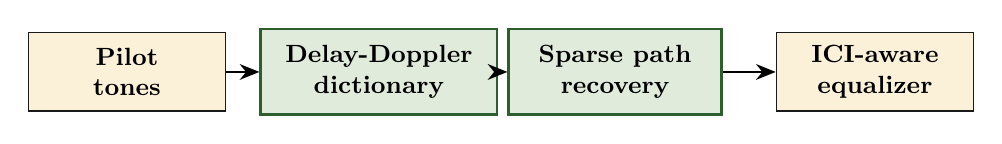
\begin{tikzpicture}[x=1cm,y=1cm]
  \node[flowbox] (pilot) at (-5.0,0) {Pilot\\tones};
  \node[method,minimum width=3.0cm] (dict) at (-1.8,0) {Delay-Doppler\\dictionary};
  \node[method,minimum width=2.7cm] (sparse) at (1.2,0) {Sparse path\\recovery};
  \node[flowbox] (eq) at (4.5,0) {ICI-aware\\equalizer};
  \draw[flowarr] (pilot) -- (dict);
  \draw[flowarr] (dict) -- (sparse);
  \draw[flowarr] (sparse) -- (eq);
\end{tikzpicture}
\end{center}
\bottomnote{Estimate the channel in a physical basis. Convert it into the OFDM ICI pattern.\\The delay-Doppler model links channel estimation and equalization.}
\end{frame}

\begin{frame}{JUNA}
\begin{itemize}\setlength{\itemsep}{0.5em}
  \item Select the sparse support explicitly
  \item Use few delay-Doppler paths:
  \[
    \vY_k=\sum_{q\in\mathcal B(k)}\bm c_{kq}s_q+\vn_k,
    \qquad
    \bm c_{kq}\text{ comes from few delay-Doppler paths.}
  \]
  \item Choose support by OMP, basis pursuit, or candidates
  \item Refine the coefficients afterwards
  \item Use reliable decoded carriers as anchors
\end{itemize}
\end{frame}

\end{document}
